\hypertarget{LinearStatistic_8c}{
\section{Linear\-Statistic.c File Reference}
\label{LinearStatistic_8c}\index{LinearStatistic.c@{LinearStatistic.c}}
}
{\tt \#include \char`\"{}party.h\char`\"{}}\par


Include dependency graph for Linear\-Statistic.c:\begin{figure}[H]
\begin{center}
\leavevmode
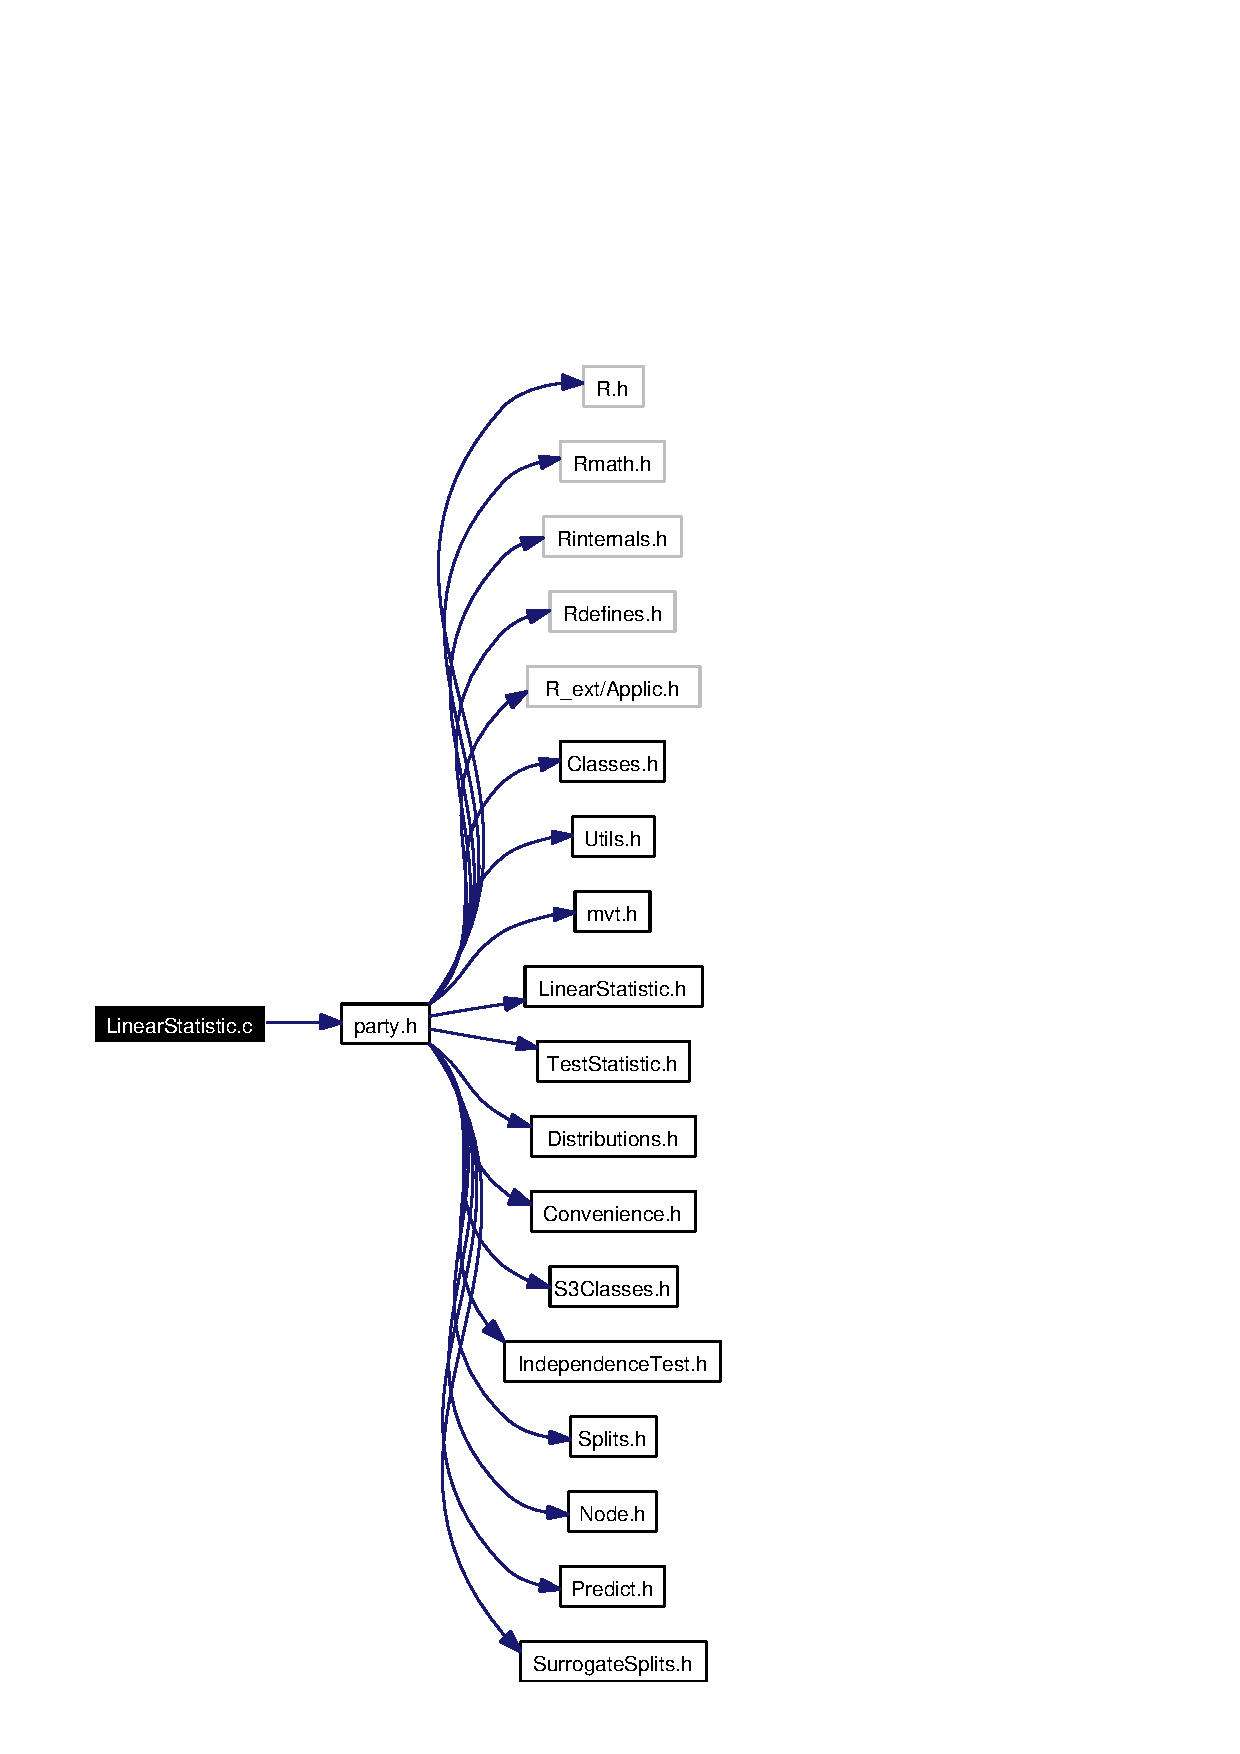
\includegraphics[width=176pt]{LinearStatistic_8c__incl}
\end{center}
\end{figure}
\subsection*{Functions}
\begin{CompactItemize}
\item 
void \hyperlink{LinearStatistic_8c_aefa2a9406bb30b323715e3db41da637}{C\_\-Linear\-Statistic} (const double $\ast$x, const int p, const double $\ast$y, const int q, const double $\ast$weights, const int n, double $\ast$ans)
\item 
SEXP \hyperlink{LinearStatistic_8c_732bfc8e1797d8953482aa31f9b43e5f}{R\_\-Linear\-Statistic} (SEXP x, SEXP y, SEXP weights)
\item 
void \hyperlink{LinearStatistic_8c_e2f62abe13ee5b625141b5d4a496d832}{C\_\-Expect\-Covar\-Influence} (const double $\ast$y, const int q, const double $\ast$weights, const int n, SEXP ans)
\item 
SEXP \hyperlink{LinearStatistic_8c_6216ea560644c08002fb32756ae67dcc}{R\_\-Expect\-Covar\-Influence} (SEXP y, SEXP weights)
\item 
void \hyperlink{LinearStatistic_8c_94a0805ea258af79d426c095feee399a}{C\_\-Expect\-Covar\-Linear\-Statistic} (const double $\ast$x, const int p, const double $\ast$y, const int q, const double $\ast$weights, const int n, const SEXP expcovinf, SEXP ans)
\item 
SEXP \hyperlink{LinearStatistic_8c_58fff8082d3ab197994a21a10c422353}{R\_\-Expect\-Covar\-Linear\-Statistic} (SEXP x, SEXP y, SEXP weights, SEXP expcovinf)
\item 
void \hyperlink{LinearStatistic_8c_a34b0f12fac36231a105d6dc903bfe89}{C\_\-Permuted\-Linear\-Statistic} (const double $\ast$x, const int p, const double $\ast$y, const int q, const int n, const int nperm, const int $\ast$indx, const int $\ast$perm, double $\ast$ans)
\item 
SEXP \hyperlink{LinearStatistic_8c_be383bcae17e8b3a1d5740ec16a9817a}{R\_\-Permuted\-Linear\-Statistic} (SEXP x, SEXP y, SEXP indx, SEXP perm)
\end{CompactItemize}


\subsection{Detailed Description}
Linear statistics for conditional inference based on Strasser \& Weber (1999)

\begin{Desc}
\item[Author:]\begin{Desc}
\item[Author]hothorn \end{Desc}
\end{Desc}
\begin{Desc}
\item[Date:]\begin{Desc}
\item[Date]2006-08-25 10:53:10 +0200 (Fri, 25 Aug 2006) \end{Desc}
\end{Desc}


Definition in file \hyperlink{LinearStatistic_8c-source}{Linear\-Statistic.c}.

\subsection{Function Documentation}
\hypertarget{LinearStatistic_8c_e2f62abe13ee5b625141b5d4a496d832}{
\index{LinearStatistic.c@{Linear\-Statistic.c}!C_ExpectCovarInfluence@{C\_\-ExpectCovarInfluence}}
\index{C_ExpectCovarInfluence@{C\_\-ExpectCovarInfluence}!LinearStatistic.c@{Linear\-Statistic.c}}
\subsubsection[C\_\-ExpectCovarInfluence]{\setlength{\rightskip}{0pt plus 5cm}void C\_\-Expect\-Covar\-Influence (const double $\ast$ {\em y}, const int {\em q}, const double $\ast$ {\em weights}, const int {\em n}, SEXP {\em ans})}}
\label{LinearStatistic_8c_e2f62abe13ee5b625141b5d4a496d832}


Conditional expectation and covariance of the influence function\par
 \begin{Desc}
\item[Parameters:]
\begin{description}
\item[{\em y}]values of the influence function \item[{\em q}]dimension of the influence function \item[{\em weights}]case weights \item[{\em n}]number of observations \item[{\em ans}]return value; an object of class `Expect\-Covar\-Influence' \end{description}
\end{Desc}


Definition at line 101 of file Linear\-Statistic.c.

References PL2\_\-covariance\-Sym, PL2\_\-expectation\-Sym, and PL2\_\-sumweights\-Sym.

Referenced by C\_\-Global\-Test(), C\_\-Lin\-Stat\-Exp\-Cov(), and R\_\-Expect\-Covar\-Influence().\hypertarget{LinearStatistic_8c_94a0805ea258af79d426c095feee399a}{
\index{LinearStatistic.c@{Linear\-Statistic.c}!C_ExpectCovarLinearStatistic@{C\_\-ExpectCovarLinearStatistic}}
\index{C_ExpectCovarLinearStatistic@{C\_\-ExpectCovarLinearStatistic}!LinearStatistic.c@{Linear\-Statistic.c}}
\subsubsection[C\_\-ExpectCovarLinearStatistic]{\setlength{\rightskip}{0pt plus 5cm}void C\_\-Expect\-Covar\-Linear\-Statistic (const double $\ast$ {\em x}, const int {\em p}, const double $\ast$ {\em y}, const int {\em q}, const double $\ast$ {\em weights}, const int {\em n}, const SEXP {\em expcovinf}, SEXP {\em ans})}}
\label{LinearStatistic_8c_94a0805ea258af79d426c095feee399a}


Conditional expectation and covariance of the a linear statistic\par
 \begin{Desc}
\item[Parameters:]
\begin{description}
\item[{\em x}]values of the transformation \item[{\em p}]dimension of the transformation \item[{\em y}]values of the influence function \item[{\em q}]dimension of the influence function \item[{\em weights}]case weights \item[{\em n}]number of observations \item[{\em expcovinf}]an object of class `Expect\-Covar\-Influence' \item[{\em ans}]return value; an object of class `Expect\-Covar' \end{description}
\end{Desc}


Definition at line 213 of file Linear\-Statistic.c.

References PL2\_\-covariance\-Sym, PL2\_\-expectation\-Sym, and PL2\_\-sumweights\-Sym.

Referenced by C\_\-Lin\-Stat\-Exp\-Cov(), and R\_\-Expect\-Covar\-Linear\-Statistic().\hypertarget{LinearStatistic_8c_aefa2a9406bb30b323715e3db41da637}{
\index{LinearStatistic.c@{Linear\-Statistic.c}!C_LinearStatistic@{C\_\-LinearStatistic}}
\index{C_LinearStatistic@{C\_\-LinearStatistic}!LinearStatistic.c@{Linear\-Statistic.c}}
\subsubsection[C\_\-LinearStatistic]{\setlength{\rightskip}{0pt plus 5cm}void C\_\-Linear\-Statistic (const double $\ast$ {\em x}, const int {\em p}, const double $\ast$ {\em y}, const int {\em q}, const double $\ast$ {\em weights}, const int {\em n}, double $\ast$ {\em ans})}}
\label{LinearStatistic_8c_aefa2a9406bb30b323715e3db41da637}


Computes the linear statistic, formula (1) in the paper\par
 \begin{Desc}
\item[Parameters:]
\begin{description}
\item[{\em x}]values of the transformation \item[{\em p}]dimension of the transformation \item[{\em y}]values of the influence function \item[{\em q}]dimension of the influence function \item[{\em weights}]case weights \item[{\em n}]number of observations \item[{\em ans}]return value; a pointer to a REALSXP-vector of length pq \end{description}
\end{Desc}


Definition at line 23 of file Linear\-Statistic.c.

Referenced by C\_\-Lin\-Stat\-Exp\-Cov(), and R\_\-Linear\-Statistic().\hypertarget{LinearStatistic_8c_a34b0f12fac36231a105d6dc903bfe89}{
\index{LinearStatistic.c@{Linear\-Statistic.c}!C_PermutedLinearStatistic@{C\_\-PermutedLinearStatistic}}
\index{C_PermutedLinearStatistic@{C\_\-PermutedLinearStatistic}!LinearStatistic.c@{Linear\-Statistic.c}}
\subsubsection[C\_\-PermutedLinearStatistic]{\setlength{\rightskip}{0pt plus 5cm}void C\_\-Permuted\-Linear\-Statistic (const double $\ast$ {\em x}, const int {\em p}, const double $\ast$ {\em y}, const int {\em q}, const int {\em n}, const int {\em nperm}, const int $\ast$ {\em indx}, const int $\ast$ {\em perm}, double $\ast$ {\em ans})}}
\label{LinearStatistic_8c_a34b0f12fac36231a105d6dc903bfe89}


Linear Statistic with permuted indices\par
 \begin{Desc}
\item[Parameters:]
\begin{description}
\item[{\em x}]values of the transformation \item[{\em p}]dimension of the transformation \item[{\em y}]values of the influence function \item[{\em q}]dimension of the influence function \item[{\em n}]number of observations \item[{\em nperm}]number of permutations \item[{\em indx}]indices for the x-part \item[{\em perm}](permuted) indices for the y-part \item[{\em ans}]return value; a pointer to a REALSXP-vector of length pq \end{description}
\end{Desc}


Definition at line 351 of file Linear\-Statistic.c.\hypertarget{LinearStatistic_8c_6216ea560644c08002fb32756ae67dcc}{
\index{LinearStatistic.c@{Linear\-Statistic.c}!R_ExpectCovarInfluence@{R\_\-ExpectCovarInfluence}}
\index{R_ExpectCovarInfluence@{R\_\-ExpectCovarInfluence}!LinearStatistic.c@{Linear\-Statistic.c}}
\subsubsection[R\_\-ExpectCovarInfluence]{\setlength{\rightskip}{0pt plus 5cm}SEXP R\_\-Expect\-Covar\-Influence (SEXP {\em y}, SEXP {\em weights})}}
\label{LinearStatistic_8c_6216ea560644c08002fb32756ae67dcc}


R-interface to C\_\-Expect\-Covar\-Influence\par
 \begin{Desc}
\item[Parameters:]
\begin{description}
\item[{\em y}]values of the influence function \item[{\em weights}]case weights \end{description}
\end{Desc}


Definition at line 171 of file Linear\-Statistic.c.

References C\_\-Expect\-Covar\-Influence(), ncol(), nrow(), PL2\_\-covariance\-Sym, PL2\_\-expectation\-Sym, and PL2\_\-sumweights\-Sym.

Here is the call graph for this function:\begin{figure}[H]
\begin{center}
\leavevmode
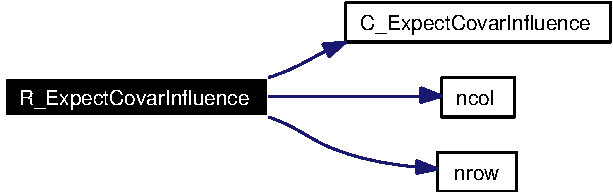
\includegraphics[width=164pt]{LinearStatistic_8c_6216ea560644c08002fb32756ae67dcc_cgraph}
\end{center}
\end{figure}
\hypertarget{LinearStatistic_8c_58fff8082d3ab197994a21a10c422353}{
\index{LinearStatistic.c@{Linear\-Statistic.c}!R_ExpectCovarLinearStatistic@{R\_\-ExpectCovarLinearStatistic}}
\index{R_ExpectCovarLinearStatistic@{R\_\-ExpectCovarLinearStatistic}!LinearStatistic.c@{Linear\-Statistic.c}}
\subsubsection[R\_\-ExpectCovarLinearStatistic]{\setlength{\rightskip}{0pt plus 5cm}SEXP R\_\-Expect\-Covar\-Linear\-Statistic (SEXP {\em x}, SEXP {\em y}, SEXP {\em weights}, SEXP {\em expcovinf})}}
\label{LinearStatistic_8c_58fff8082d3ab197994a21a10c422353}


R-interface to C\_\-Expect\-Covar\-Linear\-Statistic\par
 \begin{Desc}
\item[Parameters:]
\begin{description}
\item[{\em x}]values of the transformation \item[{\em y}]values of the influence function \item[{\em weights}]case weights \item[{\em expcovinf}]an object of class `Expect\-Covar\-Influence' \end{description}
\end{Desc}


Definition at line 306 of file Linear\-Statistic.c.

References C\_\-Expect\-Covar\-Linear\-Statistic(), ncol(), nrow(), PL2\_\-covariance\-Sym, and PL2\_\-expectation\-Sym.

Here is the call graph for this function:\begin{figure}[H]
\begin{center}
\leavevmode
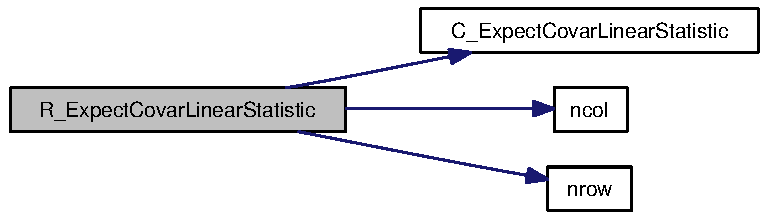
\includegraphics[width=186pt]{LinearStatistic_8c_58fff8082d3ab197994a21a10c422353_cgraph}
\end{center}
\end{figure}
\hypertarget{LinearStatistic_8c_732bfc8e1797d8953482aa31f9b43e5f}{
\index{LinearStatistic.c@{Linear\-Statistic.c}!R_LinearStatistic@{R\_\-LinearStatistic}}
\index{R_LinearStatistic@{R\_\-LinearStatistic}!LinearStatistic.c@{Linear\-Statistic.c}}
\subsubsection[R\_\-LinearStatistic]{\setlength{\rightskip}{0pt plus 5cm}SEXP R\_\-Linear\-Statistic (SEXP {\em x}, SEXP {\em y}, SEXP {\em weights})}}
\label{LinearStatistic_8c_732bfc8e1797d8953482aa31f9b43e5f}


R-interface to C\_\-Linear\-Statistic \par
 \begin{Desc}
\item[Parameters:]
\begin{description}
\item[{\em x}]values of the transformation \item[{\em y}]values of the influence function \item[{\em weights}]case weights \end{description}
\end{Desc}


Definition at line 59 of file Linear\-Statistic.c.

References C\_\-Linear\-Statistic(), ncol(), and nrow().

Here is the call graph for this function:\begin{figure}[H]
\begin{center}
\leavevmode
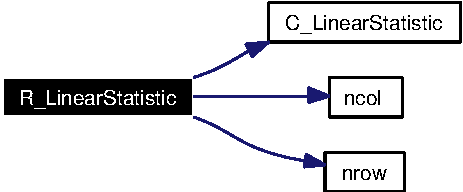
\includegraphics[width=128pt]{LinearStatistic_8c_732bfc8e1797d8953482aa31f9b43e5f_cgraph}
\end{center}
\end{figure}
\hypertarget{LinearStatistic_8c_be383bcae17e8b3a1d5740ec16a9817a}{
\index{LinearStatistic.c@{Linear\-Statistic.c}!R_PermutedLinearStatistic@{R\_\-PermutedLinearStatistic}}
\index{R_PermutedLinearStatistic@{R\_\-PermutedLinearStatistic}!LinearStatistic.c@{Linear\-Statistic.c}}
\subsubsection[R\_\-PermutedLinearStatistic]{\setlength{\rightskip}{0pt plus 5cm}SEXP R\_\-Permuted\-Linear\-Statistic (SEXP {\em x}, SEXP {\em y}, SEXP {\em indx}, SEXP {\em perm})}}
\label{LinearStatistic_8c_be383bcae17e8b3a1d5740ec16a9817a}


Linear Statistic with permuted indices\par
 \begin{Desc}
\item[Parameters:]
\begin{description}
\item[{\em x}]values of the transformation \item[{\em y}]values of the influence function \item[{\em indx}]indices for the x-part \item[{\em perm}](permuted) indices for the y-part \end{description}
\end{Desc}


Definition at line 384 of file Linear\-Statistic.c.

References nrow().

Here is the call graph for this function:\begin{figure}[H]
\begin{center}
\leavevmode
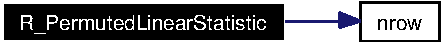
\includegraphics[width=123pt]{LinearStatistic_8c_be383bcae17e8b3a1d5740ec16a9817a_cgraph}
\end{center}
\end{figure}
